\clearpage
\subsection{Programs} % (fold)
\label{sub:what_is_a_program_}

If you are going to learn to develop software you will need to become intimately aware of what a program is. After all, as a developer you will be creating your own programs.

A program is a file that contains instructions that get the computer to perform a task. Programs are lists of commands\footnote{C and Pascal are both \emph{imperative} programming languages. In the imperative paradigm a program is seen as a list of commands instructing the computer to perform actions.} telling the computer what to do, and the order in which to do it. Each instruction is very simple, but they can be executed very quickly, allowing computers to perform quite remarkable feats.

\begin{figure}[h]
   \centering
   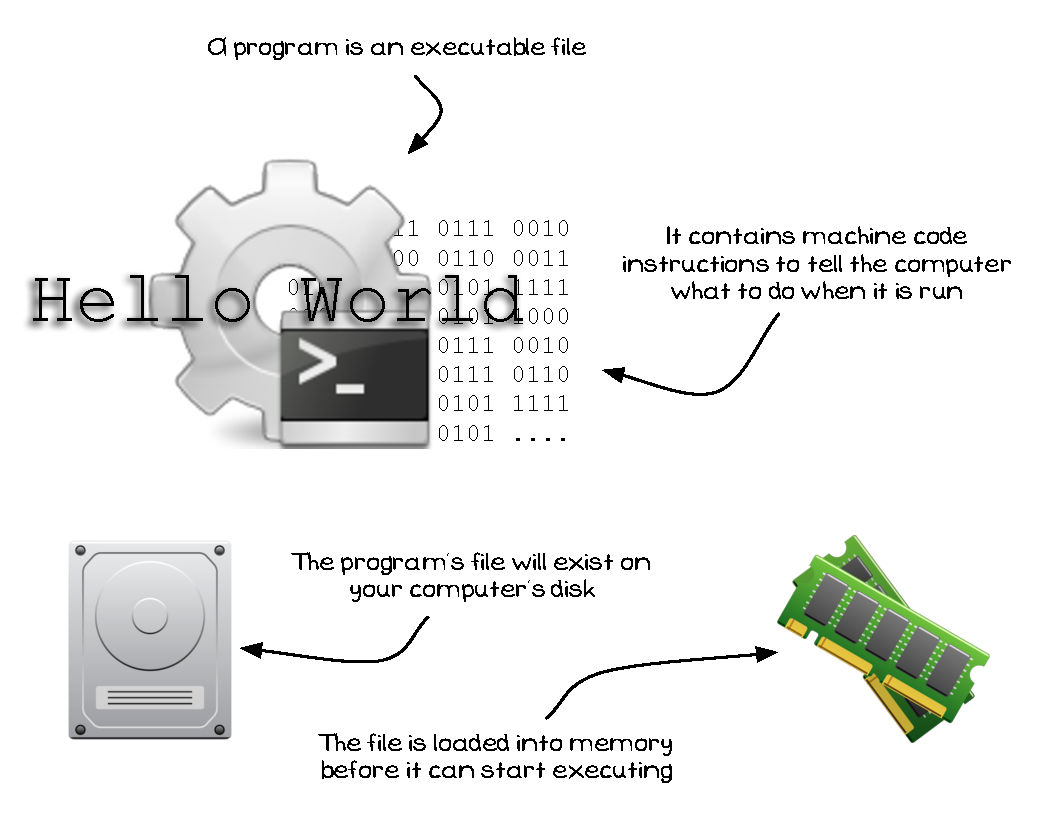
\includegraphics[width=0.9\textwidth]{./topics/programs-and-compilers/diagrams/Program} 
   \caption{A program contains instructions that command the computer to perform a task}
   \label{fig:what-is-a-program}
\end{figure}

\mynote{
\begin{itemize}
  \item You can \textbf{run} programs, which gets the computer to follow the instructions found within the program's file.
  \item To run, the program's instructions must first be loaded into memory.
  \item Once in memory, the computer starts running the instructions one after the other.
  \item When the last instruction is completed the program ends.
  \item There are several different ways to run a program:
  \begin{itemize}
    \item You can \emph{double-click} the program in a file browser.
    \item On tablets and app-phones you can \emph{tap} the program's icon.
    \item Advanced uses can enter \emph{text commands} in the Terminal to start programs.
  \end{itemize}
\end{itemize}
}

\clearpage
\subsubsection{What happens when a program runs?} % (fold)
\label{ssub:what_happens_when_a_program_runs_}

When you run a program, regardless of how it is started, the Operating System loads it from disk into memory and then starts it running. It is important that the file you try to run is a program. These are \emph{special} files that contain instructions the computer can understand.

\begin{figure}[h]
   \centering
   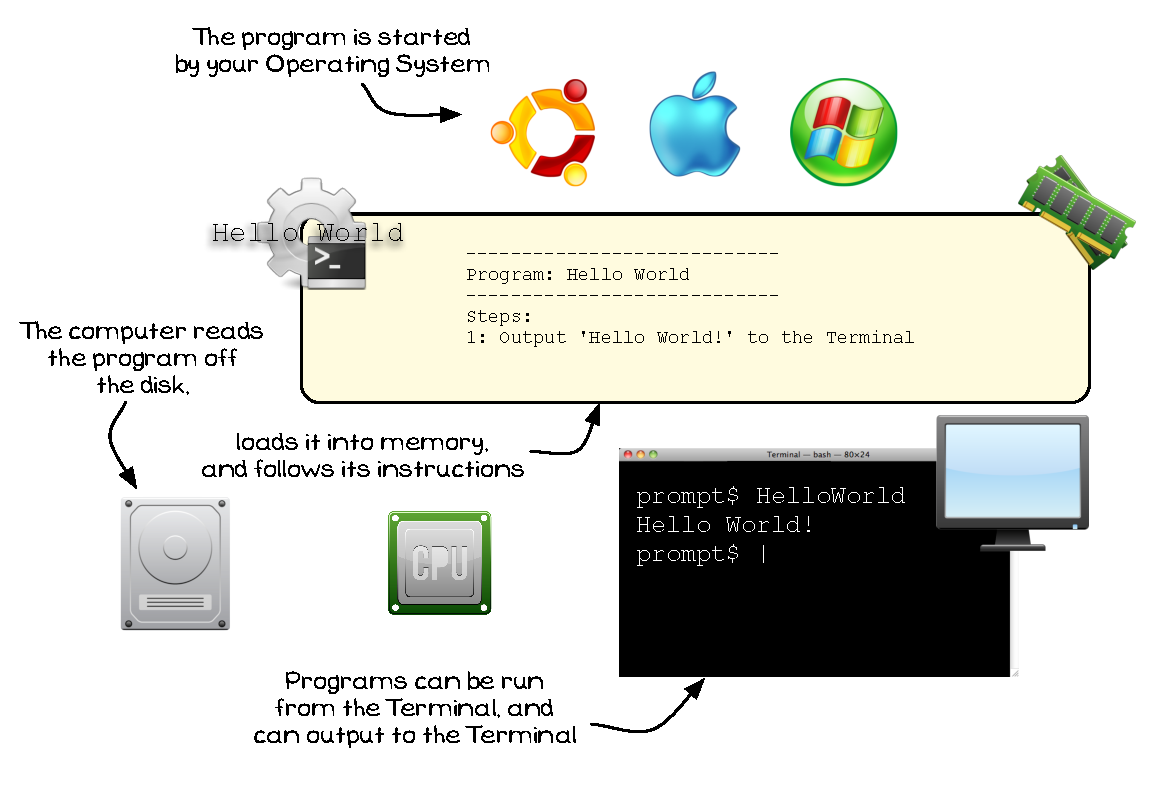
\includegraphics[width=0.9\textwidth]{./topics/programs-and-compilers/diagrams/ProgramExe} 
   \caption{Programs are loaded from disk into memory, then run}
   \label{fig:what-is-a-program-exe}
\end{figure}

\mynote{
\begin{itemize}
  \item Your Operating System is a piece of software that is responsible for managing your computer's hardware.
  \item One of the Operating System's responsible is to start programs.
  \item The \nameref{sub:terminal} can be used to start programs.
  \item Programs can also output to the Terminal.
  \item A Program must contain instructions that the computer can understand.
\end{itemize}
}

% subsubsection what_happens_when_a_program_runs_ (end)

% subsection what_is_a_program_ (end)